\part{Nivel de Transporte}
\section{Protocolos End-to-End}
Los procesos del nivel de aplicación que usan los servicios de la capa de transporte esperan que proporcione ciertos requisitos:
\begin{itemize}
  \item Garantizar la entrega de mensajes
  \item Entregar mensajes en el mismo orden en que se envían
  \item Entregar a lo sumo una copia de cada mensaje
  \item Soportar mensajes arbitrariamente grandes
  \item Soportar sincronización entre el emisor y el receptor
  \item Permitir al receptor aplicar control de flujo al emisor
  \item Soportar múltiples procesos de aplicación en cada host  
\end{itemize}
\subsection{UDP}
El protocolo de transporte más simple posible es uno que extiende el servicio de entrega de host a host de la red subyacente en un servicio de comunicación de proceso a proceso. Es probable que haya muchos procesos en ejecución en cualquier host dado, por lo que el protocolo necesita agregar un nivel de demultiplexión, lo que permite que varios procesos de aplicación en cada host compartan la red. Aparte de este requisito, el protocolo de transporte no agrega ninguna otra funcionalidad al servicio de mejor esfuerzo proporcionado por la red subyacente. El \textbf{Protocolo de Datagramas de Usuario} (User Datagrama Procol - UDP) de Internet es un ejemplo de este tipo de protocolo de transporte.

Los procesos se identifican indirectamente entre sí utilizando un localizador abstracto, generalmente llamado puerto (\textbf{port}).

La cabecera de un protocolo de extremo a extremo que implementa esta función de demultiplexación típicamente contiene un identificador (puerto) tanto para el remitente (origen) como para el receptor (destino) del mensaje. Es decir, un proceso es realmente identificado por un puerto en algún host en particular, un par \(\langle host, puerto\rangle\).

\subsubsection{Comunicación entre procesos}
\begin{figure}[H]
	\centering
	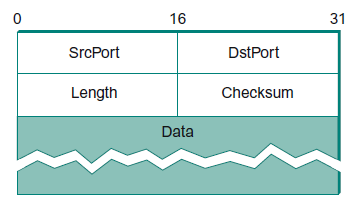
\includegraphics[width=0.5\textwidth
]{images/udp-header.png}
	\caption[Formate de Header para UDP]{Formate de Header para UDP}
	\label{fig:udp-header}
\end{figure}
Típicamente, un proceso cliente inicia un intercambio de mensajes con un proceso servidor. Una vez que el mensaje inicial esrecibido, el servidor conoce el puerto del cliente (del campo \textbf{SrcPrt} contenido en la cabecera del mensaje) y puede responderle. 

Los servidores, esperan recibir mensajes en puertos bien conocidos (\textbf{well-known ports}). Algunos ejemplos:
\begin{itemize}
  \item Los servidores de nombres de dominio (DNS) recibe mensajes en el puerto 53.
  \item El servicio de correo escucha mensajes en el puerto 25.
  \item Unix acepta mensajes en el puerto 517
\end{itemize}

Este mapeo se publica periódicamente en un RFC y está disponible en la mayoría de los sistemas Unix en el archivo /etc/services. A veces, un puerto bien conocido es solo el punto de partida para la comunicación: el cliente y el servidor usan el puerto bien conocido para acordar algún otro puerto que usarán para la comunicación posterior, dejando el puerto bien conocido libre para otros clientes.

\subsubsection{Manejo de mensajes}
\begin{figure}[H]
	\centering
	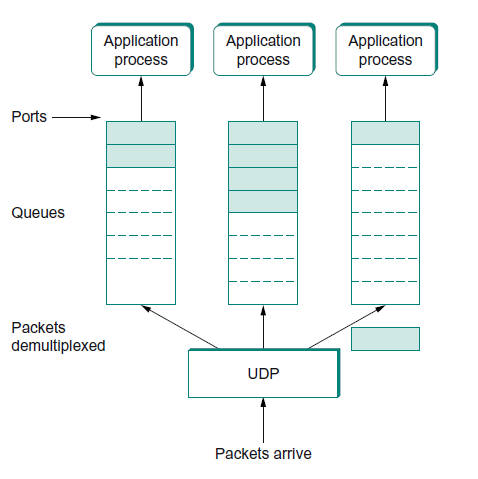
\includegraphics[width=0.5\textwidth
]{images/udp-message-queue.png}
	\caption[Cola de mensajes de UDP]{Cola de mensajes de UDP}
	\label{fig:udp-message-queue}
\end{figure}

Cuando llega un mensaje, el protocolo lo agrega al final de la cola. Si la cola está llena, el mensaje se descarta. No hay mecanismo de control de flujo en UDP para decirle al remitente que se ralentice. Cuando un proceso de aplicación desea recibir un mensaje, se elimina uno de la parte delantera de la cola. Si la cola está vacía, el proceso se bloquea hasta que haya un mensaje disponible.

Finalmente, aunque UDP no implementa el control de flujo o la entrega confiable / ordenada, también garantiza la corrección del mensaje mediante el uso de un cheksum. El mismo  toma como entrada el encabezado UDP, el contenido del cuerpo del mensaje y algo llamado \textbf{pseudoencabezado}. El pseudoencabezado consiste en tres campos del encabezado IP: número de protocolo, dirección IP de origen y dirección IP de destino, más el campo de longitud UDP. La motivación detrás de tener el pseudoencabezado es verificar que este mensaje se haya entregado entre los dos puntos finales correctos.

\subsection{Transmission Control Protocol (TCP)}
TCP garantiza la entrega confiable y en orden de un flujo de bytes. Es un protocolo full-duplex, lo que significa que cada conexión TCP admite dos flujos de bytes simulteanos en dirección opuesta. También incluye un mecanismo de control de flujo para cada uno de ellos, lo que permite al receptor limitar la cantidad de datos que el remitente puede transmitir en un momento dado. La idea de este mecanismo es limitar la velocidad a la que TCP envía datos, no por el bien de evitar que el remitente sobrecargue al receptor, sino para evitar que el remitente sobrecargue la red. Finalmente, al igual que UDP, TCP admite un mecanismo de demultiplexación que permite que varios programas de aplicación en cualquier host dado mantengan una conversación simultánea con sus pares. 

\subsubsection{Sliding Window en TCP}
TCP usa el algoritmo de ventana deslizante para asegurar la entrega confiable de los mensajes. Aunque este es el mismo algoritmo básico que vimos en la Sección \ref{sec:ventana-deslizante}, debido a que TCP se ejecuta a través de Internet en lugar de una conexión punto a punto, hay muchas diferencias importantes:
\begin{itemize}
  \item TCP admite conexiones lógicas entre procesos que se ejecutan entre dos computadoras cualquieras conectadas al Internet por lo que necesita una fase explícita de establecimiento de conexión durante la cual ambos nodos acurdan intercambiar información entre sí. Esto genera un estado compartido entre ellos que se usa para comenzar el algoritmo de ventana deslizante y que debe ser liberado cuando la conexión se cierra por lo que TCP también tiene una fase explícita de desmontaje de la conexión.
  \item Mientras que un solo enlace físico que siempre conecta las mismas dos computadoras tiene un tiempo de Round-Trip Time (RTT), las conexiones TCP probablemente tendrán tiempos de ida y vuelta diferentes dependiendo de la distancia entre ellas, la carga de la red, etc. Las variaciones en el RTT incluso son posibles durante una sola conexión TCP que dura solo unos minutos. Osea que el algoritmo de ventana deslizante debe tener un mecanismo retransmisiones con tiempos de espera adaptativos.
  \item Los paquetes pueden reordenarse a medida que cruzan el Internet. Los paquetes que están ligeramente desordenados no causan un problema ya que el algoritmo de ventana deslizante puede reordenar los paquetes correctamente usando el número de secuencia. El verdadero problema es cuán desordenados pueden estar los paquetes o, dicho de otra manera, cuán tarde puede llegar un paquete a su destino. En el peor de los casos, un paquete puede retrasarse en Internet hasta que expire el campo de tiempo de vida (TTL) de IP, momento en el cual el paquete se descarta (y, por lo tanto, no hay peligro de que llegue tarde). Sabiendo que IP descarta los paquetes después de que expire su TTL, TCP asume que cada paquete tiene un tiempo de vida máximo. El tiempo de vida exacto, conocido como tiempo de vida máximo del segmento (Maximum Segment Life - MSL), es una opción de ingeniería. La implicación es significativa: TCP tiene que estar preparado para que los paquetes muy antiguos aparezcan repentinamente en el receptor, lo que podría confundir el algoritmo de ventana deslizante.
  \item Casi cualquier tipo de computadora puede estar conectada a Internet, lo que hace que la cantidad de recursos dedicados a cualquier conexión TCP sea muy variable, especialmente considerando que cualquier host puede potencialmente admitir cientos de conexiones TCP al mismo tiempo. Esto significa que TCP debe incluir un mecanismo que cada lado usa para "aprender" qué recursos (por ejemplo, cuánto espacio de búfer) el otro lado puede aplicar a la conexión. Este es el problema de control de flujo.
\end{itemize}

\subsubsection{Formato de los segmentos}
TCP es un protocolo orientado a bytes, lo que significa que el remitente escribe bytes en una conexión TCP y el receptor lee bytes de la conexión TCP. Aunque "flujo de bytes" describe el servicio que el protocolo ofrece a los procesos de aplicación, el mismo no transmite bytes individuales a través de Internet. En cambio, en el host de origen, almacena en un búfer suficientes bytes del proceso de envío para llenar un paquete de tamaño razonable y luego envía este paquete a su par en el host de destino. En el host de destino, TCP vacía el contenido del paquete en un búfer de recepción, y el proceso de recepción lee de este búfer a su gusto.

Los paquetes intercambiados entre pares TCP se llaman segmentos, ya que cada uno lleva un segmento del flujo de bytes. Cada segmento contiene el siguiente encabezado:

\begin{figure}[H]
	\centering
	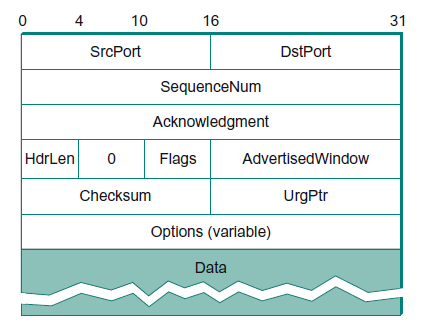
\includegraphics[width=0.5\textwidth
]{images/tcp-header.png}
	\caption[Encabezado de un paquete TCP]{Encabezado de un paquete TCP}
	\label{fig:tcp-header}
\end{figure}

\begin{itemize}
  \item \texttt{SrcPort} y \texttt{DstPort} identifican los puertos de origen y destino, respectivamente, al igual que en UDP. Estos dos campos, más las direcciones IP de origen y destino, se combinan para identificar de manera única cada conexión TCP. Es decir, la clave de demultiplexación de TCP está dada por la tupla de 4 elementos \texttt{SrcPort}, \texttt{SrcIPAddr}, \texttt{DstPort}, \texttt{DstIPAddr}.
  \item \texttt{Acknowledgment}, \texttt{SequenceNum} y \texttt{AdvertisedWindow} están involucrados en el algoritmo de ventana deslizante de TCP.
  \item \texttt{Flags} es un campo de 6 bits que se utiliza para transmitir información de control. Incluye los siguientes bits:
  \begin{itemize}
    \item \texttt{ACK} se establece cada vez que el campo \texttt{Acknowledgment} es válido, lo que implica que el receptor debe prestar atención a él. 
    \item\texttt{URG} significa que este segmento contiene datos urgentes. Cuando se establece este indicador, el segemento contiene datos urgentes desde el byte 0 hasta el byte \texttt{UrgPtr} 
    \item\texttt{PUSH} significa que el remitente invocó la operación de empuje, esto indica que el receptor debe poder leer la información contenida en el segmento apenas llegue.
    \item \texttt{RESET} significa que el receptor se ha confundido, por ejemplo, porque recibió un segmento que no esperaba recibir, por lo que desea abortar la conexión.
  \end{itemize}
  \item \texttt{Checksum} se usa exactamente de la misma manera que para UDP: se calcula sobre el encabezado TCP, los datos TCP y el pseudoencabezado, que está compuesto por los campos de dirección de origen, dirección de destino y longitud del encabezado IP. El checksum es obligatorio para TCP tanto en IPv4 como en IPv6. 
  \item \texttt{HdrLen} indica la longitud del encabezado TCP en palabras de 32 bits. Este campo también se conoce como el campo \texttt{Offset}, ya que mide el desplazamiento desde el inicio del paquete hasta el inicio de los datos.
\end{itemize}

\subsubsection{Establecimiento de una conexión TCP}
Una conexión TCP comienza con un cliente (caller) haciendo una apertura activa a un servidor (callee). Suponiendo que el servidor hubiera hecho una apertura pasiva anteriormente, los dos lados se involucran en un intercambio de mensajes para establecer la conexión. Solo después de que finalice esta fase, los dos lados pueden comenzar a enviar datos. De manera similar, tan pronto como un participante haya terminado de enviar datos, cierra una dirección de la conexión, lo que hace que TCP inicie una ronda de mensajes de terminación de conexión.

\subsubsection*{3-Way Handshake}
\begin{figure}[H]
	\centering
	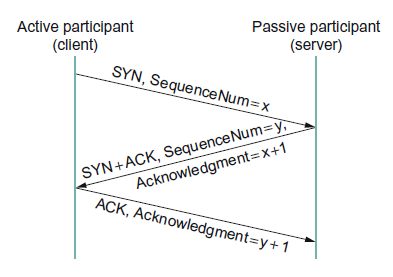
\includegraphics[width=0.5\textwidth
]{images/three-way-handshake.png}
	\caption[Intercambio de mensajes para 3-Way Handshake]{Intercambio de mensajes para 3-Way Handshake}
	\label{fig:three-way-handshake}
\end{figure}
El algoritmo utilizado por TCP para establecer y terminar una conexión se llama handshake de tres vías (Three Way Handshake).

Dos computadoras que quieran inicializar una conexión, deben acordar los números de secuencia de inicio que las dos partes planean usar para sus respectivos flujos de bytes. Primero, el cliente (el participante activo) envía un segmento al servidor (el participante pasivo) indicando el número de secuencia inicial que planea usar (\texttt{FLAG = SYN, SequenceNum = x}). El servidor responde con un solo segmento que reconoce el número de secuencia del cliente (\texttt{FLAG = ACK, Ack = x + 1}) y establece su propio número de secuencia de inicio (\texttt{Flags = SYN + ACK, SequenceNum = y}). Finalmente, el cliente responde con un tercer segmento que reconoce el número de secuencia del servidor (\texttt{Flags = ACK, Ack = y + 1}). La razón por la cual cada lado reconoce un número de secuencia que es uno más grande que el enviado es que el campo de reconocimiento realmente identifica el "siguiente número de secuencia esperado", reconociendo implícitamente todos los números de secuencia anteriores. Aunque no se muestra en esta línea de tiempo, se programa un temporizador para cada uno de los dos primeros segmentos, y si no se recibe la respuesta esperada, el segmento se retransmite.

\subsubsection{Diagrama de transición de estados de TCP}
Todas las conexiones comienzan en el estado CLOSED. A medida que la conexión avanza, la conexión se mueve de un estado a otro de acuerdo con los arcos. Cada arco está etiquetado con una etiqueta de la forma evento / acción.

\begin{figure}[H]
	\centering
	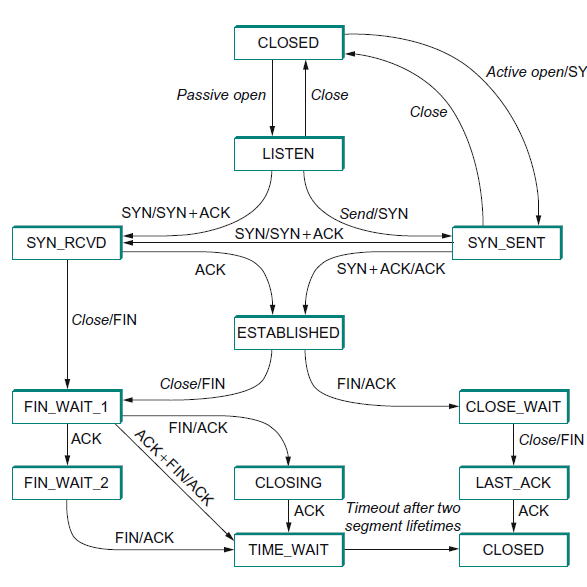
\includegraphics[width=0.5\textwidth
]{images/tcp-state-transitions.png}
	\caption[Transiciones de estado TCP]{Transiciones de estado TCP}
	\label{fig:tcp-state-transitions}
\end{figure}

\paragraph{Inicio de conexión:}Al abrir una conexión, el servidor primero invoca una operación de apertura pasiva, lo que hace que TCP se mueva al estado \texttt{LISTEN}. En algún momento posterior, el cliente realiza una apertura activa, lo que hace que su extremo de la conexión envíe un segmento \texttt{SYN} al servidor y se mueva al estado \texttt{SYN SENT}. Cuando el segmento \texttt{SYN} llega al servidor, se mueve al estado \texttt{SYN RCVD} y responde con un segmento \texttt{SYN + ACK}. La llegada de este segmento hace que el cliente se mueva al estado \texttt{ESTABLISHED} y envíe un \texttt{ACK} de vuelta al servidor. Cuando llega este \texttt{ACK}, el servidor finalmente se mueve al estado \texttt{ESTABLISHED}.

Si el \texttt{ACK} del cliente al servidor se pierde, la conexión aún funciona correctamente. Esto se debe a que el lado del cliente ya está en el estado \texttt{ESTABLISHED}, por lo que el proceso de aplicación local puede comenzar a enviar datos al otro extremo. Cada uno de estos segmentos de datos tendrá el indicador \texttt{ACK} establecido y el valor correcto en el campo de reconocimiento, por lo que el servidor pasará al estado \texttt{ESTABLISHED} cuando llegue el primer segmento de datos. Este es en realidad un punto importante sobre TCP: cada segmento informa qué número de secuencia el remitente espera ver a continuación, incluso si esto repite el mismo número de secuencia contenido en uno o más segmentos anteriores.

\paragraph{Fin de la conexión:} 
Las aplicaciones en ambos lados de la conexión deben cerrar de forma independiente su mitad de la conexión. Si solo un lado cierra la conexión, esto significa que no tiene más datos para enviar, pero aún está disponible para recibir datos del otro lado. Esto complica el diagrama de transición de estado porque debe tener en cuenta la posibilidad de que los dos lados invoquen el operador de cierre al mismo tiempo, así como la posibilidad de que primero un lado invoque el cierre y luego, en algún momento posterior, el otro lado invoque el cierre:

\begin{figure}[H]
	\centering
	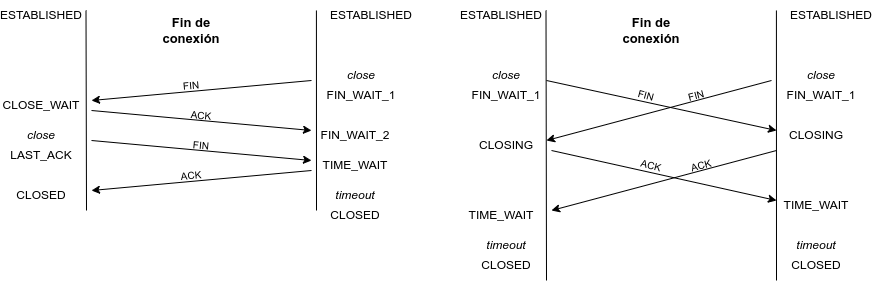
\includegraphics[width=0.8\textwidth
]{images/tcp-closing-conection.png}
	\caption[Diagrama de cierre de conexión]{Diagrama de cierre de conexión}
	\label{fig:tcp-closign-connection}
\end{figure}

Una conexión en el estado \texttt{TIME\_WAIT} no puede pasar al estado \texttt{CLOSED} hasta que haya esperado dos veces la cantidad máxima de tiempo que un datagrama IP podría vivir en Internet. La razón de esto es que, si bien el lado local de la conexión ha enviado un \texttt{ACK} en respuesta al segmento \texttt{FIN} del otro lado, no sabe si el \texttt{ACK} se entregó correctamente. Como consecuencia, el otro lado podría retransmitir su segmento \texttt{FIN}, y este segundo segmento podría retrasarse en la red. 

Si se permitiera pasar directamente al estado CLOSED, entonces otro par de procesos de aplicación podrían llegar y abrir la misma conexión (es decir, usar el mismo par de números de puerto), y el segmento \texttt{FIN} retrasado de la encarnación anterior de la misma inmediatamente iniciaría la terminación de la encarnación posterior.

\subsubsection*{Sliding Window en TCP}
La variante de TCP del algoritmo de ventana deslizante sirve para varios propósitos:
\begin{itemize}
  \item Garantiza la entrega confiable de datos,
  \item Garantiza que los datos se entreguen en orden
  \item Impone un control de flujo entre el remitente y el receptor.
\end{itemize} 

Para lograr lo último, en lugar de tener una ventana deslizante de tamaño fijo, el receptor anuncia un tamaño de ventana al remitente. Esto se hace utilizando el campo \texttt{AdvertisedWindow} en el encabezado TCP. Luego, el remitente está limitado a tener no más \texttt{AdvertisedWindow} bytes de datos no reconocidos en un momento dado. El receptor selecciona un valor adecuado para \texttt{AdvertisedWindow} en función de la cantidad de memoria asignada a la conexión con el fin de almacenar en búfer los datos. De esta manera, se evita que el remitente sobrecargue el búfer del receptor.

\subsubsection*{Envio confiable y ordenado}
El remitente mantiene un búfer de envío que utiliza para almacenar datos que se han enviado pero que aún no se han reconocido, así como datos que ha escrito la aplicación de envío pero que aún no se han transmitido.

En el lado receptor, TCP mantiene un búfer de recepción. Este búfer contiene datos que llegan desordenados, así como datos que están en el orden correcto (es decir, no faltan bytes antes en el flujo) pero que el proceso de aplicación aún no ha tenido la oportunidad de leer.

\begin{figure}[H]
	\centering
	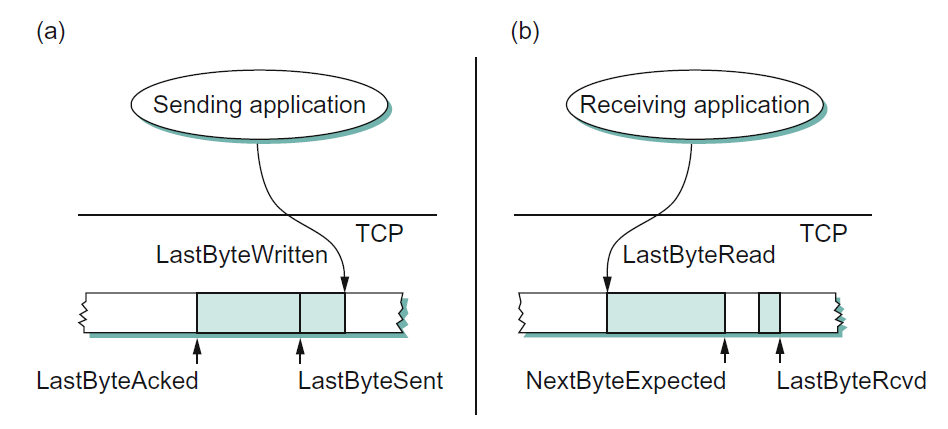
\includegraphics[width=0.8\textwidth
]{images/tcp-buffers.png}
	\caption[Buffers de TCP]{Buffers de TCP}
	\label{fig:tcp-buffers}
\end{figure}

Del lado del remitente, se mantienen tres punteros en el búfer de envío: \texttt{LastByteAcked}, \texttt{LastByteSent} y \texttt{LastByteWritten} y se cumplen las siguientes condiciones:
\begin{itemize}
  \item \(\texttt{LastByteAcked} \leq \texttt{LastByteSent}\): El receptor no puede haber reconocido un byte que aún no se ha enviado
  \item \(\texttt{LastByteSent} \leq \texttt{LastByteWritten}\): TCP no puede enviar un byte que el proceso de aplicación aún no ha escrito.
  \item Ninguno de los bytes a la izquierda de \texttt{LastByteAcked} necesita ser guardado en el búfer porque ya han sido reconocidos, y ninguno de los bytes a la derecha de \texttt{LastByteWritten} necesita ser almacenado en el búfer porque aún no se han generado.
\end{itemize}

Un conjunto similar de punteros (números de secuencia) se mantienen en el lado receptor: \texttt{LastByteRead}, \texttt{NextByteExpected} y \texttt{LastByteRcvd}. Sin embargo, las desigualdades son un poco menos intuitivas, debido al problema de la entrega desordenada:
\begin{itemize}
  \item \(\texttt{LastByteRead} < \texttt{NextByteExpected}\): Un byte no puede ser leído por la aplicación hasta que sea todos los bytes anteriores y ese mismo byte hayan sido recibidos. \texttt{NextByteExpected} apunta al byte inmediatamente después del último byte que cumple con este criterio.
  \item \(\texttt{NextByteExpected} \leq \texttt{LastByteRcvd} + 1\): Si los datos llegaron en orden, \texttt{NextByteExpected} apunta al byte después de \texttt{LastByteRcvd}, mientras que si los datos han llegado desordenados, entonces \texttt{NextByteExpected} apunta al comienzo del primer espacio en los datos.
  \item Los bytes a la izquierda de \texttt{LastByteRead} no necesitan estar en búfer porque ya han sido leídos por el proceso de aplicación local, y los bytes a la derecha de \texttt{LastByteRcvd} no necesitan estar en búfer porque aún no han llegado.
\end{itemize}

\subsubsection*{Control de flujo}
Ambos búferes mencionados en la sección anterior son de algún tamaño finito, denotados como \texttt{MaxSendBuffer} y \texttt{MaxRcvBuffer}.

En TCP, el receptor se debe asegurar qué \[\texttt{LastByteRcvd} - \texttt{LastByteRead} \leq \texttt{MaxRcvBuffer}\]
para evitar la sobrecarga de su búfer. Para esto, controla el tamaño de la ventana deslizante que anuncia al remitente seteando el campo \texttt{AdvertisedWindow} en el encabezado TCP con el valor \[\texttt{MaxRcvBuffer} - ((\texttt{NextByteExpected}-1)-\texttt{LastByteRead})\]
que es la cantidad de espacio libre que tiene en el búfer.

A medida que le llegan los datos, los reconoce siempre que también hayan llegado todos los bytes anteriores. Además, \texttt{LastByteRcvd} se mueve a la derecha (se incrementa), lo que significa que la ventana anunciada potencialmente se reduce. Si se reduce o no depende de qué tan rápido el proceso de la aplicación local está consumiendo datos. Si el proceso local está leyendo datos tan rápido como llegan, entonces la ventanta anunciada se mantiene. Sin embargo, si el proceso receptor se atrasa, tal vez porque realiza una operación muy costosa en cada byte de datos que lee, entonces la ventana anunciada se vuelve más pequeña con cada segmento que llega, hasta que eventualmente llega a 0.

\paragraph{Wraparound:} El número de secuencia utilizado en una conexión determinada podría dar la vuelta, un byte con el número de secuencia \(x\) podría enviarse en un momento determinado, y luego en un momento posterior un segundo byte con el mismo número de secuencia \(x\) podría enviarse. Nuevamente, asumimos que los paquetes no pueden sobrevivir en Internet por más tiempo que el \(MSL\) recomendado. Si esto sucede o no depende de qué tan rápido se pueden transmitir los datos a través de Internet, es decir, qué tan rápido se puede consumir el espacio de número de secuencia de 32 bits.

\paragraph{Manteniendo el pipe lleno:} El valor del \texttt{AdvertisedWindow} debe ser lo suficientemente grande como para permitir que el remitente mantenga el pipe lleno. El receptor es libre de no anunciar una ventana de tamaño máximo (tan grande como lo permite el campo \texttt{AdvertisedWindow}).

El máximo \texttt{AdvertisedWindow} posible se puede calcular como el  producto de la demora y el ancho de banda \(delay\times bandwidth\).

\subsubsection{Transmisión de datos}
TCP usa tres mecanismos para decidir cuando transmitir datos:
\begin{itemize}
  \item TCP mantiene una variable, generalmente llamada \textbf{tamaño máximo de segmento}\\ (\(MSS\)), y envía un segmento tan pronto como ha recopilado \(MSS\) bytes del proceso de envío. 
  Generalmente se establece este valor de tal manera de evitar que la IP local se fragmente.Es decir, \(MSS\) se establece en la unidad máxima de transmisión (MTU) de la red conectada directamente, menos el tamaño de los encabezados TCP e IP.
  \item TCP admite una operación de empuje, y el proceso de envío invoca esta operación para vaciar efectivamente el búfer de bytes no enviados.
  \item El último disparador para transmitir un segmento es que se active un temporizador; el segmento resultante contiene tantos bytes como los que están actualmente almacenados en búfer para su transmisión.
\end{itemize}

\paragraph{Silly Window Syndrome:} Supongamos que el remitente está acumulando bytes para enviar, pero la ventana está actualmente cerrada. Ahora suponga que llega un \texttt{ACK} que abre efectivamente una ventana de pocos bytes. La especificación original no aclaraba que hacer en esta situación y las primeras implementaciones de TCP decidieron transmitir un segmento medio lleno. Después de todo, no hay forma de saber cuánto tiempo pasará antes de que la ventana se abra aún más.

Resulta que esta estrategia de aprovechar agresivamente cualquier ventana disponible conduce a una situación ahora conocida como el \texttt{síndrome de la ventana tonta}.

Si el remitente llena agresivamente un contenedor vacío más pequeño que un \(MSS\) tan pronto como llega, el receptor \(ACK\) ese número de bytes, y por lo tanto el contenedor introducido en el sistema permanece en el sistema indefinidamente. Es decir, se llena e inmediatamente se vacía en cada extremo y nunca se fusiona con contenedores adyacentes para crear contenedores más grandes.

Actualmente, se puede retrasar este sindromehaciendo que el receptor espere a poder aceptar \(MSS\) bytes antes de anunciar una ventana abierta.

Dado que no podemos eliminar la posibilidad de que se introduzca un contenedor pequeño en el flujo, también necesitamos mecanismos para fusionarlos. El receptor puede hacer esto retrasando los ACK: enviando un ACK combinado en lugar de varios más pequeños, pero esta es solo una solución parcial porque el receptor no tiene forma de saber cuánto tiempo es seguro esperar a que llegue otro segmento o para que la aplicación lea más datos.

\paragraph{Algoritmo de Naggle:} Mientras TCP tenga datos en vuelo, el remitente eventualmente recibirá un ACK. Este ACK se puede tratar como un temporizador que se activa, lo que desencadena la transmisión de más datos. El algoritmo de Nagle proporciona una regla simple y unificada para decidir cuándo transmitir:
\begin{itemize}
  \item[] La aplicacion produce \(b\) bytes:
  \begin{itemize}
    \item[] Si \(b \geq  MSS\) y \(\texttt{AdvertisedWindow}\geq MSS\)
     \begin{itemize}
      \item[] Se manda un segmento completo
    \end{itemize}
    \item[] Sino:
    \begin{itemize}
      \item[] Si hay datos que todavia no fueron reconocidos (sin acks)
      \begin{itemize}
        \item[] Acumular datos hasta que el próximo \texttt{ACL} llegue.
      \end{itemize}
      \item[] Sino:
      \begin{itemize}
        \item[] Enviar todos los datos ahora
      \end{itemize}
    \end{itemize}
  \end{itemize}
\end{itemize}

En otras palabras, siempre está bien enviar un segmento completo si la ventana lo permite. También está bien enviar inmediatamente una pequeña cantidad de datos si actualmente no hay segmentos en tránsito, pero si hay algo en vuelo, el remitente debe esperar un ACK antes de transmitir el siguiente segmento.

Debido a que algunas aplicaciones no pueden permitirse tal retraso para cada escritura que realiza en una conexión TCP, la interfaz de socket permite a la aplicación desactivar el algoritmo de Nagel estableciendo la opción TCP \texttt{NODELAY}. Usar esta opción significa que los datos se transmiten lo antes posible.

\subsubsection{Retransmisión adaptativa}
Debido a que TCP garantiza la entrega confiable de datos, retransmite cada segmento si no se recibe un \texttt{ACK} en un cierto período de tiempo. El protocolo establece este tiempo de espera como una función del RTT que espera entre los dos extremos de la conexión. Desafortunadamente, dada la gama de RTT posibles entre cualquier par de hosts en Internet, así como la variación en RTT entre los mismos dos hosts con el tiempo, elegir un valor de tiempo de espera apropiado no es tan fácil. Para abordar este problema, TCP utiliza un mecanismo de retransmisión adaptativo.

\paragraph{Algortimo original:} Cada vez que TCP envía un segmento de datos, registra el tiempo. Cuando llega un ACK para ese segmento, TCP lee el tiempo nuevamente y luego toma la diferencia entre estos dos tiempos como un \texttt{SampleRTT}. TCP luego calcula un \texttt{EstimatedRTT} como un promedio ponderado entre la estimación anterior y esta nueva muestra. Es decir,
  \[ \texttt{EstimatedRTT} = \alpha\times \texttt{EstimatedRTT} + (1-\alpha)\times \texttt{SampleRTT} \]

El parámetro \(\alpha\) se selecciona para suavizar el \texttt{EstimatedRTT}. Un \(\alpha\) pequeño realiza un seguimiento de los cambios en el RTT, pero tal vez esté demasiado influenciado por fluctuaciones temporales. Por otro lado, un \(\alpha\) grande es más estable pero quizás no sea lo suficientemente rápido como para adaptarse a cambios reales. La especificación original de TCP recomendó una configuración de \(\alpha\) entre \(0.8\) y \(0.9\).

TCP luego usa \texttt{EstimatedRTT} para calcular el tiempo de espera de una manera bastante conservadora:
\[ \texttt{TimeOut} = 2\times \texttt{EstimatedRTT}\]

\paragraph{Algoritmo de Karn/Partridge:} Un ACK no reconoce realmente una transmisión; en realidad, reconoce la recepción de datos. En otras palabras, cada vez que se retransmite un segmento y luego llega un ACK al remitente, es imposible determinar si este ACK debe asociarse con la primera o la segunda transmisión del segmento con el fin de medir el tiempo de ida y vuelta de la muestra. Es necesario saber qué transmisión asociar con el fin de calcular un \texttt{SampleRTT} preciso.  

Este algoritmo, resuelve esto haciendo que solo se calcule un \texttt{SampleRTT} para segmentos que fueron transmitidos una sola vez. Cada vez que TCP retransmite un segmento, duplica el valor del siguiente timeout (usa \textbf{exponential backoff}). Esta última decisión se debe a que la congestión es la causa más probable de segmentos perdidos, lo que significa que el remitente de un mensaje no debe reaccionar agresivamente a un timeout. De hecho, cuanto más veces se agota el tiempo de espera de la conexión, más cautelosa debe ser la fuente.

\paragraph{Algoritmo de Jacobson/Karels:} Es una mejora al algoritmo anterior. Si la variación entre las muestras es pequeña, entonces el \texttt{EstimatedRTT} puede ser considerado confiable y no hay razón para multiplicar esta estimación por 2 para calcular el timeout. Por otro lado, una gran varianza en las muestras sugiere que el valor de timeout no debe estar demasiado acoplado al \texttt{EstimatedRTT}. Para tener en cuenta estas situaciones, una vez obtenido un \texttt{SampleRTT}, se calcula el \texttt{TimeOut} de la siguiente manera:
\[\texttt{Difference} = \texttt{SampleRTT} - \texttt{EstimatedRTT}\]
\[ \texttt{EstimatedRTT} = \texttt{EstimatedRTT} + (\delta\times\texttt{Difference})\]
\[Deviation = Deviation + (\delta\times(|\texttt{Difference}| - \texttt{Deviation}))\]
\[\texttt{TimeOut} = \mu\times\texttt{EstimatedRTT} + \phi\times\texttt{Deviation}\]

Donde \(\delta\) es una valor valor entre 0 y 1. \(\mu = 1\) y \(\phi=4\).  De esta manera, si la varianza es pequeña, el \texttt{Timeout} es cercano al \texttt{EstimatedRTT}, y si la varianza es grande, entonces \texttt{Deviation} domina el calculo.

\newpage

% Traducir del ingles
account. Intuitively, if the varia
tion
among samples is small, then the EstimatedRTT can be better trusted
and there is no reason for multiplying this estimate by 2 to compute the
timeout. On the other hand, a large variance in the samples suggests that
the timeout value should not be too tightly coupled to the EstimatedRT
% Al español:
Intuitivamente, si la variación entre las muestras es pequeña, entonces el \texttt{EstimatedRTT} puede ser mejor confiable y no hay razón para multiplicar esta estimación por 2 para calcular el tiempo de espera. Por otro lado, una gran varianza en las muestras sugiere que el valor de tiempo de espera no debe estar demasiado acoplado al \texttt{EstimatedRTT}.

